\chapter{System Design}
\label{cha:fourth_chapter}

In this chapter we will present the approaches we have developed to solve the problem of classifying and localize the different diseases on a given Chest X-Ray. We will first talk about the approach we used to deal with uncertain labels, then we will present the models that we've developed to identify the different pathologies and we'll show the techniques that have been used to aggregate them. Finally, we will talk about the approach we've used to identify the region of the CXR affected by the disease. 


\section{Uncertain Labels}
\label{sec:uncertainty}
As already introduced in Chapter \ref{cha:third_chapter}, the dataset contains a significant number of diseases that have been labelled as uncertain. The uncertainty could reflect both an unreliable diagnosis or an ambiguity in the report. In their work, Irvin et al. \cite{irvin2019chexpert}, proposed different policies to deal with them:
\begin{itemize}
    \item U-Ignore: this is the simplest approach, that consists in ignoring all the uncertain labels during the training. This method, however, could produce biased models and also reduce the effective size of the dataset if the number of uncertain labels is significant.
    \item U-Zeros: this approach consists in assigning a 0 label to the uncertain one, thus considering the associated disease as not present.
    \item U-Ones: this is similar to the previous method but, instead of considering the uncertain labels as negative, they are considered as positive, thus they are assigned a label equal to 1.
    \item U-SelfTraining: with this method, the uncertain labels are first considered as unlabeled examples. Then a model is  trained using the U-Ignore policy and, finally, it is used to make predictions in order to re-label each uncertain label.
    \item U-MultiClass: the last policy treats the \textit{u} label as its own class. Thus, for each pathology, three different probabilities $\{p_{0} , p_{1},p_{u}\}$ are carried out, each one representing the probability of belonging to, respectively, class $0$, $1$ or $u$.
\end{itemize}

Focusing our attention on U-Zeros and U-Ones policy, Pham et al. \cite{pham2019interpreting}, in their work, put the evidence on a problem related to these two approaches: mapping all the uncertainty to either 0 or 1 will certainly result in a lot of wrong labels and, consequently, the model would be misguided during training. Thus, they used a technique called \ac{LSR}, introduced by Szegedy et al. \cite{lsr}, that allows to exploit the large amount of uncertain labels but preventing the model from becoming over confident about the prediction of examples that could contain mislabeled data.
Thus, the U-Ones policy has been modified by mapping each uncertain label to a random number close to 1. Formally, we have:
\begin{equation}
\scalebox{1.2}{
$
\bar{y}_{k}^{(i)} = \left\{\begin{matrix}
x, & \hfill \textup{if} \; y_{k}^{(i)}  = u\\ 
y_{k}^{(i)}, &\hfill  \textup{otherwise}
\end{matrix}\right.
$
}
    \label{eq:equation_4.1}
\end{equation}

\noindent where $x \sim U(a_{1},b_{1})$ is a randomly distributed number between $a_{1}$ and $b_{1}$. Similarly, the U-Zeros policy can be modified, mapping the uncertain labels to a number $x \sim U(a_{1},b_{1})$ close to 0.

\section{Convolutional Neural Network}
\label{sec:cnn}
In this section we talk about the first approach we've used, involving Artificial Neural Network. We start by describing the simplest model we've used and gradually we'll show how we have improved it.

\subsection{Single CNN And Training Procedure}
\label{sec:single_cnn}
The first approach we have investigated is the one involving a Convolutional Neural Network trained with U-Ones policy and \ac{LSR} (presented in the previous section). The uncertain labels, thus, have been mapped to a random number uniformly sampled between the interval $[0.55,0.85]$.

\vspace{3mm}
\subsubsection{Network Architecture}

\noindent Instead of training a Neural Network from scratch, we have decided to rely on Transfer Learning, using a Neural Network previously trained on a different dataset and retraining it in order to adapt to our new task. The architecture we used is the same already employed by Irvin et al. in their previous works \cite{irvin2019chexpert} \cite{rajpurkar2017chexnet}, called DenseNet121 and introduced for the first time in 2016 by Huang et al. \cite{densenet}. The peculiarity of this architecture is the use of dense connections that prevent the problem of vanishing information as the depth of the network increases. This problem is addressed by connecting each layer directly to each other in order to ensure the maximum information flow between them. Thus a layer receives the input from all the preceding layers and passes its own output to all the subsequent ones, as we can see in the example in Figure \ref{fig:figure_4.1} 

\begin{figure}[htbp!]
\centering
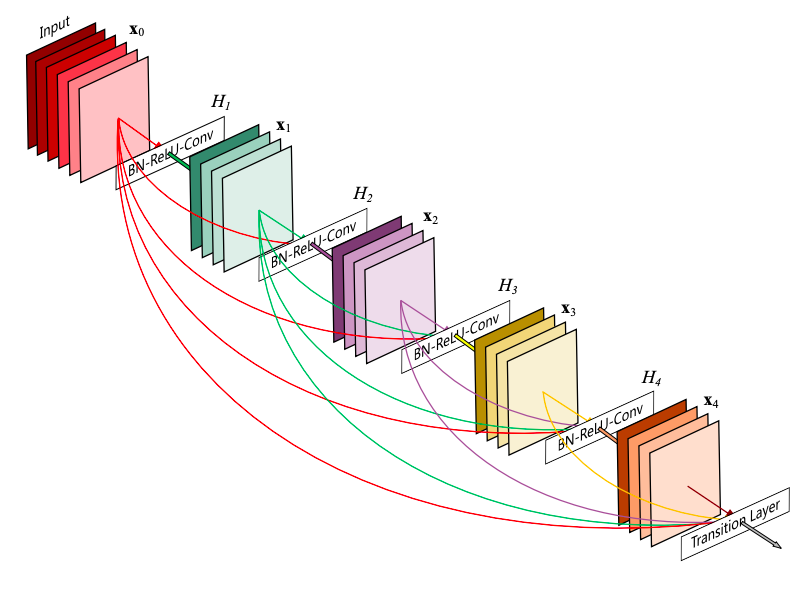
\includegraphics[scale=0.45]{Tesi/images/densenet}
\caption{Densely Connected Neural Network}
\label{fig:figure_4.1}
\end{figure}

The weights of the network have been initialized with that of the same network trained on the ImageNet dataset. The Fully Connected layer has been removed and substituted by a Global Average Pooling followed by a new \ac{FC} layer (note that the \ac{GAP} is essential for the production of a Class Activation Map).
The last layer produces a 14-dimensional output, after which we have applied an elementwise sigmoid function. If we call $z_{k}$ the output corresponding to the k-th label, the result of applying a sigmoid is: 
\vspace{3mm}

\begin{equation}
    y_{k} = \frac{1}{1+ exp(-z_{k})} , k = 1 \dots 14
    \label{eq:eq_4.2}
\end{equation}
\vspace{3mm}

\noindent The sigmoid function allows to squeeze $z_{k}$ in a range between $[0,1]$, thus we can give to $y_{k}$ a probabilistic interpretation.
\noindent Figure \ref{fig:figure_4.2} summarizes the overall network architecture:


\begin{figure}[htbp!]
\centering

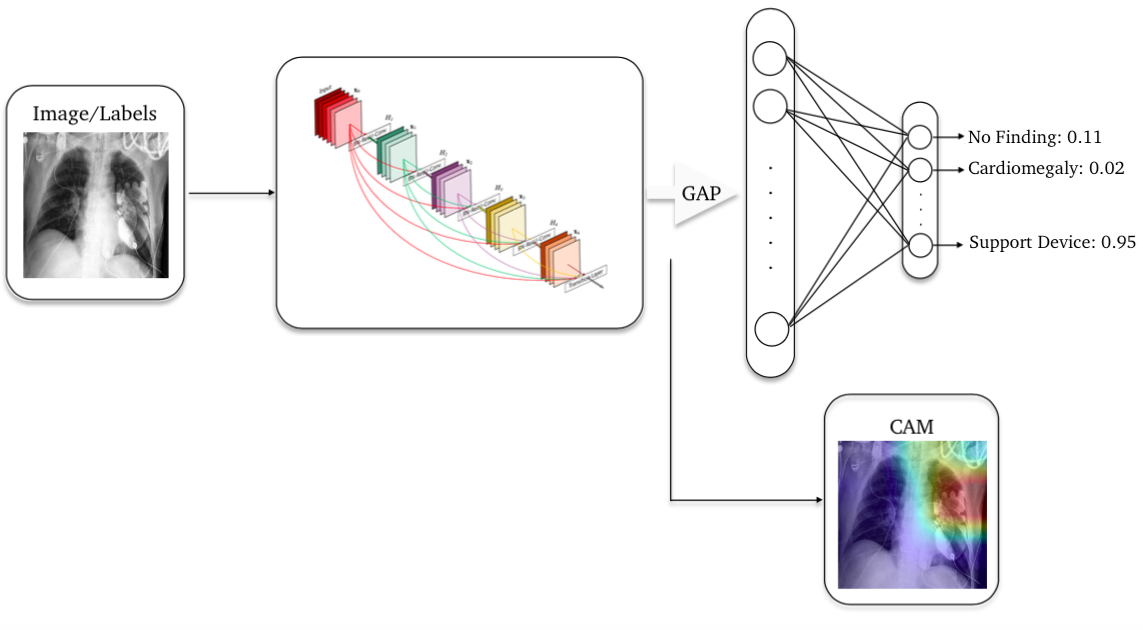
\includegraphics[scale=0.37]{Tesi/images/Architecture}
\caption{Network Architecture}
\label{fig:figure_4.2}
\end{figure}



\vspace{5mm}

\subsubsection{Training}

\noindent The network has been trained using Adam optimization algorithm \cite{adam} with default parameters $\beta_{1} = 0.9$ and  $\beta_{2} = 0.999$. The learning rate was initially set to $1e-4$ and then it has been gradually reduced by a factor of 10 at each epoch, allowing large weights changes at the beginning of the learning process and small changes towards the end. The number of epochs has been set to 10, but we also allowed the algorithm to early stop in case the optimization process show no more improvement on the validation set during the last 4 epochs. The objective function minimized by the optimizer is the binary cross entropy loss between the ground-truth labels and the predicted ones, who's formulation is the the following: 
\vspace{3mm}
\begin{equation}
\scalebox{1.1}{
    $l(\boldsymbol{\theta}) = \sum_{i=1}^{N} \sum_{k=1 }^{14} y_{k}^{(i)} \textup{log}  \hat{y}_{k}^{(i)} + (1-y_{k}^{(i)}) \textup{log} (1-\hat{y}_{k}^{(i)} )$
    }
    \label{eq:eq_4.3}
\end{equation}

\noindent where $\boldsymbol{\theta}$ are the weights, $\hat{y}_{k}^{(i)}$ is the prediction associated to the i-th sample for class k and $y_{k}^{(i)}$ is its corresponding ground truth.
Finally, after the data have been preprocessed following the steps described in section \ref{sec:preprocessing}, they have been batched using a batch size of 64 and they have been shuffled in order for the data to be independent and identically distributed.

\subsection{Conditional Training}
\label{sec:conditional_training}
As introduced in Section \ref{sec:dataset_content} the labels are organized according to a hierarchy (Figure \ref{fig:figure_3_1}). In the model we have defined in the previous section, however, we did not incorporated this knowledge, omitting an information that, instead, should be leveraged in order to help the model to better discriminate among the different diseases. The approach we are going to show has been proposed by Pham et al. in \cite{pham2019interpreting}. 

\vspace{5mm}

The proposed algorithm is divided in two phases. The first one is called \textit{conditional training} and it's goal is to learn the dependency among parent and child labels. This can be done by training the classifier on data presenting only positive parent-level labels, teaching it to distinguish the lower-level ones (Figure \ref{fig:figure_4.3}). During the second phase, instead, the classifier will be fine tuned using the whole dataset, in this way it learns to classify also the parent-level labels, that could either be positive or negative. This is accomplished by freezing all the layers of the pretrained network except for the last fully connected one and training it again. 


\begin{figure}[htbp!]
\centering

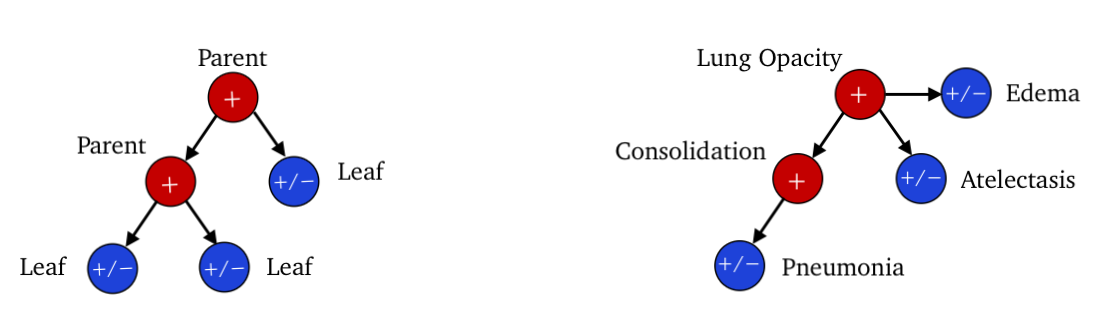
\includegraphics[scale=0.37]{Tesi/images/Conditional Training.png}
\caption[Conditional Training Example]{The left figure shows the key idea behind conditional training. In the right one there is an example, in which the classifier is trained on samples containing only positive instances of \textit{Lung Opacity} and \textit{Consolidation} in order to classify the child labels \textit{Edema}, \textit{Atelectasis} and \textit{Pneumonia}.}
\label{fig:figure_4.3}
\end{figure}

Using this training strategy, the output of the network can be viewed as the conditional probability that a label is positive giving its parent label being positive. Our goal, however, is to predict the unconditional probability. In order to do that we can rely on Bayes Theorem, calculating the probability of each label being positive by multiplying each conditional probability produced by network along the path from the root to the current node.
For example, considering the tree depicted in Figure \ref{fig:figure_4.4}, where $\boldsymbol{\alpha}$ and $\boldsymbol{\beta}$ are parent labels, while  $\boldsymbol{\gamma}$  and  $\boldsymbol{\delta}$ are leaf:

\newpage

\begin{figure}[htbp!]
\centering

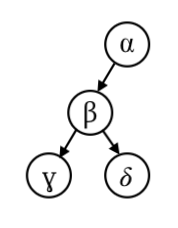
\includegraphics[scale=0.5]{Tesi/images/CT_inference.png}
\caption{Example of tree presenting four diseases}
\label{fig:figure_4.4}
\end{figure}

\noindent The network provides the conditional probabilities $p(\alpha)$, $p(\beta|\alpha)$, $p(\gamma|\beta)$, $p(\delta|\beta)$. The unconditional predictions for labels $\boldsymbol{\gamma}$  and  $\boldsymbol{\delta}$, instead, are given by: 

\begin{equation}
\begin{split}
    p(\boldsymbol{\gamma}) = p(\boldsymbol{\alpha})p(\boldsymbol{\beta}|\boldsymbol{\alpha})p(\boldsymbol{\gamma}|\boldsymbol{\beta})\\[7pt]
 p(\boldsymbol{\delta}) = p(\boldsymbol{\alpha})p(\boldsymbol{\beta}|\boldsymbol{\alpha})p(\boldsymbol{\delta}|\boldsymbol{\beta})
 \end{split}
    \label{eq:eq_4.4}
\end{equation}

\noindent Note that this approach ensures that the probability of presence of a disease for a child label is always smaller than that of its parent.

\subsection{Neural Network Ensemble}
\label{sec:nn_ensemble}
In Chapter \ref{cha:second_chapter} we have talked about Ensemble, a widely used Machine Learning technique who's aim is to gather the predictions coming from different classifiers and combine them in order to enhance the quality of the predictions.

\vspace{5mm}

In a multilabel classification setting it's hard to obtain high results for each target using a single classifier and, often, the score for each label varies with the choice of the architecture. So we decided to rely on Embedding, trying to combine several weak classifiers into a stronger one. Again, instead of building our own architecture from scratch, we used some of the most popular pretrained network emplyoed for image classification tasks. The list of the network we have used, along with some information about their structure, is shown in Table \ref{table:table_4.1}

\newpage

\begin{table}[h!]
\centering
\begin{tabular}{|l|l|l|l|l|} 
\hline
\textbf{Name}     & \textbf{\#Parameters} & \hfill\textbf{Depth} & \hfill\textbf{Size} & \hfill\textbf{Year}  \\ 
\hline
DenseNet121       & \hfill7M                    & \hfill121               &  \hfill33MB             & \hfill2016 \cite{densenet}              \\
DenseNet169       & \hfill12,5M                 & \hfill169               &   \hfill57MB            &     \hfill2016 \cite{densenet}           \\
DenseNet201       & \hfill18M                   & \hfill201              &   \hfill80MB           &        \hfill2016 \cite{densenet}        \\
InceptionResNetV2 & \hfill54M                   & \hfill572             &      \hfill215MB         &      \hfill2016 \cite{inceptionresnetv2}          \\
Xception          & \hfill21M                   &  \hfill126              &     \hfill88MB          &    \hfill2016 \cite{xception}            \\
VGG16             & \hfill15M                   &   \hfill23             &   \hfill528MB            &  \hfill2014 \cite{vgg16}               \\
VGG19             & \hfill20M                   &   \hfill26             &    \hfill549MB           &      \hfill2014 \cite{vgg16}           \\
\hline
\end{tabular}
\caption{List of pretrained CNN used}
\label{table:table_4.1}
\end{table}

All the Networks have been trained following the same approach used for the training of DenseNet121 (described in Section \ref{sec:single_cnn}). At the end of the training process, thus, we had 7 classifiers, each one carrying out a different set of predictions. We will now talk about the approaches we investigated to combine them.

\vspace{5mm}

\noindent\scalebox{1.4}{\textbf{Average}}

\vspace{2mm}

\noindent The first (and simplest) approach we have used consist in averaging the predictions made by the classifiers. If we indicate with $y_{i}(\mathbf{x})$ the 14-dimensional output of classifier $i$, then the final prediction $\tilde{y}(\mathbf{x})$, computed using the predictions coming from all the $N$ classifiers, is given by:  

\begin{equation}
    \centering
    \tilde{y}(\mathbf{x}) = \frac{1}{N}\sum_{i=1}^{N} y_{i}
    \label{eq:eq_4.5}
\end{equation}

\vspace{3mm}

\noindent The main drawback of this approach, however, is that it gives the same importance to all the models, without taking care of the fact that some classifiers may outperform other in classifying some diseases and, thus, their opinion should have a higher weight in the process of carrying out the final prediction.

\vspace{7mm}

\noindent\scalebox{1.4}{\textbf{Weighted Average}}

\vspace{2mm}

\noindent We tried to overcome the problem that arose using a simple average aggregation by using a different weight for each model. The weights have been assigned using an heuristic we developed that is based on the concept of Entropy. In Information Theory the Entropy is a quantity associated to a random variable that capture the level of uncertainty related to its possible outcome. For example, consider tossing a coin: in the case in which the coin is fair (i.e head and tail have both the same probability to occur), we are very insecure about the result, thus in this case the entropy is maximum. If, instead, the coin is not fair and one result has a higher probability to occur than the other, the result will be less uncertain and, consequently, the entropy will be lower.
We used this quantity to measure the level of uncertainty of each outcome. Consider, for example, the prediction $p_{i}$ for label $i$, taken out by a given model. We can compute the entropy of the predicions as: 

\begin{equation}
    H(p_{i}) = - p_{i} \log _{2}p_{i} - \left(1-p_{i} \right) \log _{2}\left( 1-p_{i} \right)
    \label{eq:eq_4.6}
\end{equation}

\noindent Note that, if $H(p_{i})$ captures the information related to the uncertainty of a prediction, $(1-H(p_{i}))$, instead, gives us an insight related to how safe the model is about it.

\noindent Now that we have introduced the concept of entropy we can describe how we used it in our task. Consider a \ac{CXR} given as input to our $N=7$ predictors. The output associated to the $L=14$ labels can be represented as a matrix: 

\begin{equation}
P =
\begin{bmatrix} 
    p_{11} & \dots & p_{1L} \\
    \vdots & \ddots & \vdots\\
    p_{N1} &  \dots      & p_{NL} 
\end{bmatrix}
\label{eq:eq_4.7}
\end{equation}

\noindent where $p_{ij}$ is the predictions carried out by i-th model for label $j$. Using equation \ref{eq:eq_4.6} we can also compute a matrix of weigths:

\begin{equation}
H =
\begin{bmatrix} 
    h_{11} & \dots & h_{1L} \\
    \vdots & \ddots & \vdots\\
    h_{N1} &  \dots      & h_{NL} 
\end{bmatrix}
\label{eq:eq_4.8}
\end{equation}

\vspace{4mm}

\noindent Now, the final prediction $y_{i}$ for label $i$ can be calculated as a weighted average of all the outputs, where a weight captures the certainty of the model with respect its own prediction. Here's the mathematical formulation: 

\begin{equation}
y_{i} = \sum _{k=1}^{N} \left(1- h_{ki} \right)p_{ki}
\label{eq:eq_4.9}
\end{equation}

\vspace{7mm}

\noindent\scalebox{1.4}{\textbf{Stacking}}

\vspace{2mm}

\noindent The last aggregation approach we investigated is the one involving Stacking, a technique already presented in Section \ref{sec:ensemble}. The idea is to let an algorithm learn the best way to combine the predictions instead of doing it manually. 
We have used the predictions generated over our validation set as input to train a meta-learner, who's aim is that of aggregating the outputs in order to generate the final prediction. Note that in order to train the meta-learner it's very important to use data that have not been employed during the training of the base classifiers, otherwise we would incur in overfitting.
The predictions coming from all the networks have been stacked together, thus the size of a single example was constituded by $L \times N$ data points, where $L$ is the number of labels and $N$ the number of predictors.
As meta-learner we used a Random Forest algorithm, whose hyperparameters have been tuned using a Grid Search approach.

\section{Embedding}
\label{sec:nn_embedding}
The inherent ability of \acp{CNN} to deal with images made them a standard for the task of \acp{CXR} analysis. In this section, however, we try to investigate other approaches that can be used to classify the pathologies. For many algorithms, however, it's almost impossible to learn the discriminative features directly from the image, unless it has a very small size. It would be useful, then, to have a small representation of the \ac{CXR} that, however, is able to capture all the meaningful informations nedeed by the algorithm. Neural Networks can provide us such a representation by using a technique called Embedding, presented in section \ref{sec:embedding}. When the input image is processed by the network, indeed, it pass through a sequence of layers who's aim is to extract the meaningful features that are subsequently used to feed the fully connected classifier. During this process, moreover, the image is downsampled by the pooling layer, thus its spatial size is reduced as it flows through the layers. So, if we cut the network at a certain point, the output we observe is a representation of the original input embedded into a lower dimensional space. 
In our work we have extracted the embedding using the Neural Networks we trained described in Section \ref{sec:nn_ensemble} (note that each model provided us a different embedding). All the Networks have been cut at the same point, that is immediately after the Global Average Pooling layer, producing a one-dimensional vector. Table \ref{table:table_4.2} provides an insight about the shape of the embedding for each model:


\begin{table}[h!]
\centering
\begin{tabular}{|l|l|} 
\hline
\textbf{Model Name}         &   \hfill \textbf{Embedding Shape}\\
\hline
DenseNet121 &   \hfil (1,1024) \\\hline
DenseNet169 &  \hfil (1,1664)   \\\hline
DenseNet201 &  \hfil (1,1920) \\\hline
InceptionResNetV2 &  \hfil (1,1536) \\\hline
Xception &  \hfil (1,2048) \\\hline
VGG16 &  \hfil (1,512) \\\hline
VGG19 &  \hfil (1,512) \\\hline

\end{tabular}
\caption{Embedding Shape}
\label{table:table_4.2}
\end{table}

\subsection{Random Forest}
\label{sec:random_forest_model}
Once we've extracted the embeddings, they can be used as input for other models. The first approach we have explored is that involving Random Forest. As introduced in Chapter \ref{cha:first_chapter}, Random Forest is a learning algorithm that combines a group of decision trees and aggregates their output. 
Since the embeddings we had were different from each other, we decided to train a different Random Forest for each one of them. Using the validation set, we have optimized the hyperparameters by means of a Grid Search algorithm, that is an exhaustive search through a manually specified subset of values. The following hyperparameters have been taken into consideration: 
\begin{itemize}
    \item \textbf{Number of estimators}: the number of tree in the forest. Due to computational reason it has been set 200 for all our models.
    \item \textbf{Max features}: number of features to consider when looking for the best split (for each model we set it equal to the square root of the total number of variables).
    \item \textbf{Max depth}: maximum depth of the trees. The deeper the tree, the more precise it is, but this could lead to overfitting.
    \item \textbf{Min sample split}: minimum number of samples required to split an internal node.
    \item \textbf{Min sample leaf}: minimum number of samples required to be at a leaf node.
\end{itemize}

\noindent Table \ref{table:table_4.3} contains a summary of hyperparameters we used for each model.

\begin{table}[h!]
\centering
\begin{tabular}{|l|l|l|l|l|} 
\hline
\textbf{Model Name} &   \hfil \textbf{Max Depth}&   \hfil \textbf{Min Sample Split}&   \hfil \textbf{Min Sample Leaf}\\
\hline
DenseNet121 &       \hfil15  &   \hfil2 &   \hfil10  \\\hline
DenseNet169 &       \hfil15  &   \hfil2 &   \hfil10  \\\hline
DenseNet201 &       \hfil30  &   \hfil10 &   \hfil10  \\\hline
InceptionResNetV2&  \hfil30  &   \hfil10 &   \hfil1  \\\hline
Xception    &       \hfil30  &   \hfil10 &   \hfil1  \\\hline
VGG16       &       \hfil 5  &   \hfil2 &   \hfil 10 \\\hline
VGG19       &       \hfil15  &   \hfil50 &   \hfil 1 \\
\hline
\end{tabular}
\caption{Random Forest Hyperparameters}
\label{table:table_4.3}
\end{table}


\noindent Once the models have been trained, we combined their predictions using the same approaches discussed in the previous section (simple average, weighted average with entropy and stacking).


\subsection{XGBoost}
\label{sec:xgboost_model}
The last approach we tried is the one involving XGBoost (eXtreme Gradient Boosting) \cite{xgboost}, that is an efficient implementation of Gradient Boosting, introduced in section \ref{sec:gradient_boosting}. As already mentioned, this algorithm iteratively improves the predictions, adjusting them by making a step in the direction minimizing the loss function, which is given by the gradients.
We trained a different classifier for each one of the embedding we extracted from our Neural Networks and we combined their predictions using the same approaches described in the previous section.
In order to prevent overfitting, we constrained the structure of the trees, setting the maximum depth to 3 and then we trained each models for 50 rounds. 



\section{Class Activation Map}
\label{sec:class_activation_map}
As previously stated, the goal of this work is double: predicting the probability, for a given pathology, to be present on a \ac{CXR} and also localize it. Up to this moment we focused the attention on the first task, thus we want now to talk about the second one. 
The Neural Networks we trained allowed us to extract the Class Activation Map, that is the area that the model predicts to be the most indicative of each observation.The activation maps have been generated following the methodology proposed in \cite{cam_paper} and illustrated in Section \ref{sec:cam}: given a trained \ac{CNN}, the \ac{CAM} can be computed by making a weighted sum of the feature maps extracted by the last convolutional layer. Since we trained many models, we were able to compute multiple Class Activation Maps and, as already made during the classification task, combine them in order to improve the quality. However it would have made no sense to aggregate indiscriminately all of them, because we would risk to combine a map produced by a model predicting the absence of a pathology with one coming from a model telling the opposite. Thus we have decided to merge only the heatmaps coming from models having the same prediction over the presence or absence of the disease. 

\subsection{Bounding Box Generation}
\label{sec:bounding_box}
Once we have generated the \ac{CAM}, we used them to automatically generate a bounding box surrounding the area associated to the pathology. In order to do that, we first used the Class Activation Map as a mask to determine the salient area of the image. In order to do that, we have converted each pixel of the \ac{CAM} to a binary value, using the following rule:
\begin{equation}
    b(x,y) = \left\{\begin{matrix}
1, & \textup{if CAM(x,y)} \geq  threshold 
\\ 
0, & \textup{if CAM(x,y)} < threshold 
\end{matrix}\right.
\label{eq:cam_mask}
\end{equation}

where $b(x,y)$ is the intensity value of a pixel at position $(x,y)$. The threshold, instead, has been computed as:

\begin{equation}
   threshold = \alpha \times max(\textup{CAM}), \alpha \in \left[0,1\right]
   \label{eq:threshold}
\end{equation}

Once we got the mask, it has been overlapped to the original image $I$, and the saliency region $p(x,y)$ has been extracted by making a pointwise product:

\begin{equation}
  p(x,y) = I(x,y) \cdot b(x,y)
   \label{eq:saliency_region}
\end{equation}

Once we got that image, we were able to extract the coordinates of its contours and, using them, we draw the bounding box over the original image. Figure \ref{fig:figure_4.5} shows the full process used to automatically extract the bounding box. The first figure contains the original \ac{CXR}, the second one shows the generated \ac{CAM}, the third one represents the saliency region $p(x,y)$ extracted using the heatmap and, finally, the last one shows the automatically generated bounding box.

\begin{figure}[htbp!]
\centering
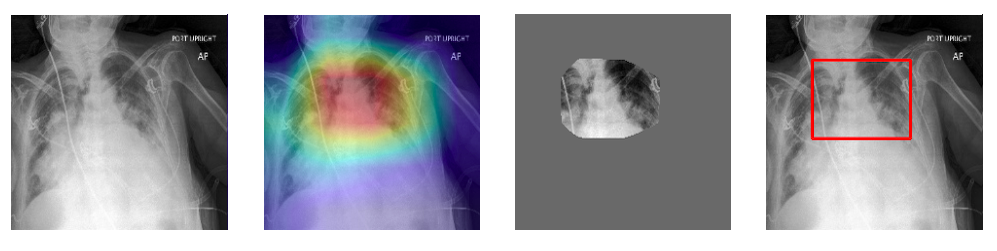
\includegraphics[scale=0.43]{Tesi/images/bbox.png}
\caption{Bounding Box Generation}
\label{fig:figure_4.5}
\end{figure}

\section{Summary}
\label{sec:chapter_4_summary}
In this chapter we have shown all the techniques we have used to solve the problems of predicting and localizing the different diseases. We started showing how to better deal with the uncertain labels, then we have built the first model that, gradually, we have modified, trying to improve the overall predictions perfomances. Finally we have shown the ability of the trained models to localize the pathologies on the \ac{CXR} and how this localization ability can be used to automatically generate a bounding box sorrounding the region interested by the pathology. In the next chapter we will talk about the metrics we used to evaluate our models and we'll exhibit and discuss the results we achieved.